\chapter{Introduction}
\epigraph{Three can keep a secret, if two of them are dead.}{Benjamin
  Franklin}

This book is about finding secrets that were present in computer
systems, sent over the Internet or a wireless network, or
inadvertently left in a digital document. 

Over the years a wide variety of programs running on many different
kinds of computers have been responsible for significant privacy
violations. The violations are typically \emph{unintentional}---the
people who wrote these programs didn't create them with the goal of
violating privacy. Instead, the programs have had bugs that caused
private information to be inadvertently retained or distributed. The
bugs are typically so subtle that most people using the program don't
realize that their private information is potentially being
compromised. And because the private information leaked by these bugs
is typically embedded in a form that is invisible or easily ignored,
the bugs can persist for weeks, months, or even years before they are
discovered and fixed.

\section{Technical Privacy Auditing}

This book describes some of the ways that private information has been
leaked in modern information systems and explains how you could have
found those leaks using tools that are freely available. We call this
process ``technical privacy auditing'' because it uses technical
tools to find privacy problems in software.

Most of the technical privacy failures that we know about were not
discovered by the companies that wrote the software in
question. Instead, the bugs were typically discovered by students,
journalists, and computer enthusiasts---people who looked at the data
and saw something that they thought just didn't belong. 
The basic premise of this book is that many such privacy snafus can
be discovered through straightforward visual inspection. The goal of
this book is to teach you to understand what you are looking at, so
that you will be in a position to discover new privacy violations in
the future.

The root cause of many technical privacy violations is the complexity
of modern information systems. Today's computers are vast, with
gigabytes of storage, tens of thousands of application programs, and
real-time connections to data networks that continually download ever 
more code and data. A typical cell phone with 16 gigabytes of memory can
store literally hundreds of thousands of digital photographs, hours of
video, or months of audio recorded from its internal
microphone. It's very easy for a programmer to overlook some small
piece of storage that may hold some very sensitive piece of
information. 

\subsection{Notable Privacy Leaks}

For example, in April 2011 two security researchers discovered that
Apple's iOS~4 operating system was tracking the movements of every
iPhone and iPad and storing that information in a database on the
mobile device. This database was copied to the users'
desktop or laptop computer whenever they backed up their mobile
device. Pete Warden and Alasdair Allan discovered
the file by accident while they were working on a project to create
visualizations called \emph{heat maps}. The two were apparently
looking for geospatial information that they could visualize with
their software then they stumbled upon a large database of such data
in the iPhone's backup
files~\cite{apple-tracking}. The two developed an application that
took the data and plotted it on a map, with larger dots indicating
more data points~(\figref{heatmap}). A media uproar resulted---fueled
in no small part by Warden and Allan's program, which allowed anyone
with an iPhone to see precisely where they had been tracked. 
Apple later released a
statement stating that the database was
not the user's locations, but the location of nearby wireless access
points that was used by the iPhone's location services to determine
the phone's position. Apparently the phone downloaded this information
as it moved around to aid in real-time geolocation without the need to
use the phone's built-in GPS. The fact that the database was never cleared and
continued to be updated even when the phone's location services was
disabled was a ``bug,'' according to Apple---a bug that was fixed
shortly after it was publicized by Warden and Allan~\cite{apple-tracking-statement}. 

\begin{figure}
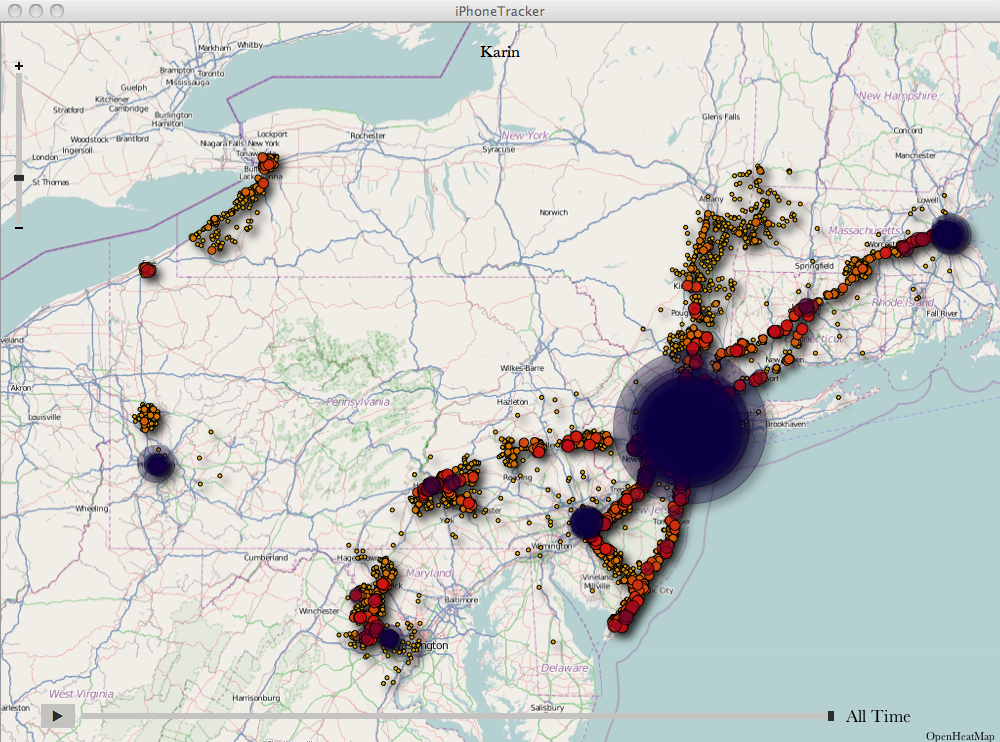
\includegraphics[width=\textwidth]{ch-1/5637893141_ba59f2d989_o.png}
\caption{In April 2011 two researchers discovered that Apple's iOS 4
  operating system recorded the location of nearby Wi-Fi access points
  to aid in geolocation. Due to a bug the database was never
  cleared. As a result, the database could easily be used to create a
  map of every place that the iPhone had been. (C) 2011 John
  Niedermeyer. {\small (Licensed under Creative Commons
  Attribution-NonCommercial-ShareAlike 2.0 Generic)}}.\label{heatmap}
% http://www.flickr.com/photos/nedward/5637893141
\end{figure}

Privacy leaks such as Apple's are insidious because they are
invisible both to users and to the companies that produce
hardware and software. Sometimes these problems result when a program
developed for a small group of technical users is deployed to a user
base that is largely and less technically inclined. Other times they
are simply bugs and technical oversights that were not detected when
the program was developed because nobody looked deeply at the data. 

Other examples of privacy leaks include:
\begin{itemize}
\item Microsoft leaking windows registration information (cite)
\item VA Laptop
\item In May 2013 a firm called Decipher Forensics revealed that Snapchat, an application that sends photos with a
  self-destruct timer, didn't actually delete photos as
  promised. Instead the program simply renamed the photos so that they
  could not be seen with normal tools on the telephone\cite{ksl-snap-chat}.
\end{itemize}

\subsection{Personally Identifiable Information?}
Most of the leaks described in the previous section share a common
theme: each involved the collection and possible release of personally
identifiable information (PII).

*EXPLAIN WHAT IT IS*

\subsubsection{Legal definitions}

\subsubsection{Practical definitions}

\subsection{Practical Concerns}
\subsubsection{Reuse of identifiers - at the same time, at different times}
\subsubsection{Shared IDs}
\subsubsection{specificity of identifiers; birthday problem}
\subsubsection{IP addresses}
\subsubsection{Identifiers: IPv4, IPv6, Mobile ID, SIM cards, Phone \#s, email addressses}
\subsection{GUIDs and identifiers}
\subsection{What is ``Unique''}

\section{Digital Forensics Tools}

This book describes how to find leaks of personal information using
digital forensics tools. The previous section gave a brief description
of different kinds of 


The tools that this book introduces for technical privacy auditing are
commonly used for digital forensics and for data
  recovery. \emph{Digital forensics} is a branch of forensic sciences
  that involves the investigation of material found on digital
  devices. Digital Forensics \emph{examiners} employ a variety of
  tools and techniques to find information that might be useful for
  solving a crime, understanding an electronic break-in, or simply
  establishing if information has been stolen or inappropriately
  accessed. 


all too easy for a program to inadvertently collect a piece of private
information and then leave it in memory, save it in a file, or send it
over a network. 

Programs can have privacy-related bugs for years without being noticed 

have been 

Modern computers are extraordinarily complex systems with vast amounts
of storage, high-performance network connections, and all kinds of
sensors. Today a 

Since the dawn of the consumer Internet in the 1990s there have been
many cases in which sensitive information was inadvertently released
because a computer program did not behave properly. 

The secrets are typically
private information that was created and or distributed with a
computer program. 


Over the past 
Typically some user trusted the program to protect
their privacy but it didn't. by a piece
of software that was trusted by their users to protect their privacy
but which failed to do so. We know about 

someone trusted, but that acted in program se secrets were not put
there intentionally---they 

. Specifically, this book is about
finding secrets that are \emph{hidden}, \emph{invisible}, or simply
easy to \emph{overlook}. Secrets that shouldn't be present, but
are. Secrets that are present in computer systems, sent over
information networks, or .

Many 

\section{Privacy and Public Policy }

\subsection{Non-Technical Privacy Audits}

\subsection{Allowable Leaks}

\section{Unnoticed data leakage - why it's a problem}
\subsection{Example: Geolocation Data in JPEGs}
  - Show how to find where a photo was taken with Preview on a Mac. 
\subsection{Example: Blacked out text in PDFs}
EEOC

Senate committee

\section{Detecting data leakage as an experimental science}
\subsection{Detecting data leakage attempts to prove a negative}


Examples in this book should run on Windows, Macintosh and Linux-based
systems. The code was largely developed on a Mac, which is similar to
Linux. 

\section{Conventions used in this book}
In general this book follows \emph{Wikipedia Manual of
  Style}\footnote{\url{http://en.wikipedia.org/wiki/Wikipedia:Manual_of_Style}}
and specifically the Computer
Science\footnote{\url{http://en.wikipedia.org/wiki/Wikipedia:WikiProject_Computer_science/Manual_of_style}}
  and
  Computing\footnote{\url{http://en.wikipedia.org/wiki/Wikipedia:Manual_of_Style/Computing}}
  sections. Specific conventions useful in understanding this book are
  described below.

\subsection{Fonts}

Text in this book is generally typeset in the serif font that you are
now reading. The fixed-width courier font is used for programs,
computer input and output, as well as for numbers that might
reasonably be expected to be constants in a computer program. Thus,
the Earth is 150 million kilometers (150 Gm) from the sun, but a
traditional disk sector has |512| bytes (|512|~B).

\subsection{Radix}
Numbers are generally assumed to be in base 10 unless otherwise
specified. Binary digits will be suffixed with a |b|; octal
is indicated with a leading |0| as in the case in most programming
languages; hexadecimal numbers will have a suffix of an |h| in text
but may be prefixed with |0x| or |\x|. Unfortunately there are
exceptions which must be inferred from context. For example, hex dumps
and cryptographic hashes are always presented courier as unadorned hexadecimal
digits. Examples are shown in \tabref{nomen}.

\begin{table}
\begin{tabular}{rlcrl}
     &              &         & Decimal  \\
Base & Nomenclature & Example & Equivalent      & Usage \\
\hline
2  & Binary      &  |10101111b|& 175            & Text\\
\hline
8  & Octal       &  |0377|     & 255            & Text and code\\
8  & Octal       &  |\377|     & 255            & Code\\
10 & Decimal     &  |1234|     & 1234           & Text and code\\
16 & Hexadecimal &  |DEADBEEFh|& 3,735,928,559  & text \\
   &             &  |0xFF|     & 255            & Output \\
   &             &  |\xFF|     & 255            & Python code\\
\end{tabular}
\caption{Examples of numbers in various bases used in this book.}
\end{table}

\subsubsection{Units}

Natural phenomena discussed in this book are described in Metric
units. Manufactured objects are described in either Metric units or
United States customary units, depending on the system of measurements
that was used to design and produce the object, with approximate
metric units indicated as appropriate. Thus, this book
discusses 5.25-inch (133mm) floppy disks.

\subsection{SI and IEC Multipliers}\label{sec:si-and-iec}
% \note{1MB = 1,000,000 bytes}
% \note{1MiB = 1,048,576 bytes}

Today there are two standards in computing for representing sizes of
files, storage systems, and memory banks: SI (the International System
of Units) decimal prefixes and IEC (International Electrotechnical
Commission) binary prefixes. This situation is confusing because until
recently the SI prefix names \emph{kilo}, \emph{mega} and \emph{giga} were commonly used
for both decimal and binary notation, the correct multiplier being
inferred from usage. Today there is an effort underway to clarify
usage. This section describes correct usage and provides hints for
determining when usage is incorrect.

SI decimal prefixes are commonly used to represent metric
quantities. For example, the SI prefix \emph{giga} multiplies the value that follows by
$10^9$; thus a gigabyte (GB) is
$10^9=1,000,000,000$ bytes. (Confusingly, this is called a billion bytes
in the US but a thousand million bytes in Great Britain, although the
Oxford Dictionary English (British Edition) that ships with MacOS 10.8
calls such usage ``dated.'')

The IEC prefix \emph{gibi} multiples the value following by $2^{30}$. A \emph{gibibyte}
(GiB) is thus $2^{30}=1,073,741,824$ bytes. This has been proper usage
since 1999 when the IEC adopted standard 60027-2 for binary prefixes.

The confusion dates back to the early days of computing, when the ``K''
and ``M'' prefixes were commonly used to mean 1,024 and 1,048,576
when describing memory systems but 1,000 and 1,000,000 when
describing mass storage systems. The difference in terminology resulted
from the way that these systems were addressed. Memory was addressed
by a series of binary address lines, while electromechanical drums and
disks were addressed by specifying a head, a track, and then counting
sector numbers: such numbers only map to even powers-of-two when the
number of heads, tracks and sectors are also even powers-of-two, and
this is rarely the case due to manufacturing concerns.

For much of computing history the correct sense of Ks and Ms could be
inferred from context and, in any event, the difference between 1000
and 1024 wasn't all that significant.

The difference in interpretation became an issue in the 1990s as the
number of people using computers mushroomed and as the commonly used
prefixes went from Ks to Ms and then Gs, resulting in a larger
divergence between the power-of-two measurement and the corresponding
power-of-ten measurement. The IEC prefixes were proposed in
1996\cite{iec:1996},
published as an international standard in 1999, and adopted by the
International Standards organization with the addition of prefixes for
describing exbi (Ei=$2^{60}$), zebi (Zi=$2^{70}$) and yobi (Yi=$2^{80}$) byte
quantities in 2006\cite{iec:80000-13:2008}.  

Despite this standardization effort, today we live in a somewhat
confusing world in which so-called ``4GB'' DRAM modules 
store precisely 4,294,967,296 bytes
but ``4GB'' microSD cards sold for cell
phones store 4,000,000,000 bytes. Even more confusing, the DRAM
module may have four ($2^{2}$) chips, each storing 1073741824
($2^{30}$) bytes each, while the microSD card may two million flash
pages, each with 4096 bytes of usable storage, but present that
information as precisely 7,812,500 logical 512-byte blocks.  These
differences are the result of different operational requirements for
the two kinds of memory, resulting in different kinds of access
electronics, different kinds of software, and different economics. 

It is likely that the IEC binary prefixes will show increased use
with time. Therefore this book uses them to describe block size and
sector size, since they are typically multiples of 512 ($2^9$), but 
SI decimal prefixes are used to describe disk sizes, since that is the way
the devices are sold to consumers.



\section{Python}
This book makes extensive use of the Python programming language for
its examples. All of the examples are tested under Python~3.3,
although Python~2.7 may work with most of the demonstration programs
as well.  This section describes specific aspects of the Python
programming language that are important in our examples and that may
be missed in an introductory Python programming class.

\subsection{Reading and Writing Files: Binary vs.\ Text}

When a Python program opens a file that file may be opened in one of
two modes: \emph{text} or \emph{binary}.  When opened as text, Python
assumes that the files contain text characters that have been encoded
with an appropriate codec---for example, that they are Unicode files
coded as UTF-8. Assuming such a codec qcan cause problems when reading
binary data, since many binary combinations do not represent valid
characters. To avoid this problem, files will normally be opened in
binary mode. This is done by opening files with method
|open(filename,"rb")|.

\subsection{Python's struct.unpack}
Much of the information on computers is stored as binary encoded
values. Such values can be easily read and written using python's
|struct.unpack| method, which reads a binary structure and returns a
python tuple of the decoded values.  

The binary structure is decoded using a \emph{format
  specification}. For example, this Python fragment will print the
decimal value of the hex string DEADBEEFh:

\lstinputlisting[caption=A program to print the decimal value of the hexadecimal number \texttt{DEADBEEFh}]{intro/deadbeef.py}


\subsection{Path Delimiter}
Windows uses the backslash (|\|) as a path delimiter, while Unix
systems use the forward slash (|/|). In general this is not a problem,
because Python run on Windows will treat either slash as a path
delimiter. So in general, this book will use the forward slash as a
path delimiter, even for code that runs on Windows-based computers.

\subsection{Accessing Raw Devices}

A ``raw'' device is a device file that can be opened by user programs
like a normal file but reads and writes are sent directly to the
underlying physical device. Typically access to the raw disk devices 
requires administrative privileges, since access to the raw device
bypasses the computer's operating system.

To access the physical drives on a Windows computer open the hidden
physical drives |\\.\PhysicalDrive0| through
|\\.\PhysicalDriveNN|. To open the physical drive for reading use use
mode |rb|, for writing use the ``updating'' mode |rb+|. List the
physical drives on your Windows system with the command:

\begin{code}
c:\ (@ \hl{wmic diskdrive list brief /format:list} @)
\end{code}

Unix-based systems associate two pseudo-files in the |/dev/| directory with
each physical device; additional pseudo-files map to disk
partitions. Macs use |/dev/diskNN| for block devices and
|/dev/rdiskNN| for raw devices. Partitions are identified by appending
a |sJ|, where |J| is the partition number.  List the physical drives
on a Mac with the command:

\begin{code}
$ (@ \hl{ls -l /dev/disk*} @)
\end{code}
%$

Linux systems name block devices |/dev/sdA| where |A| is a letter |a|
through the highest device letter; partitions are identified with an
appended letter. Modern Linux systems also map physical devices in
additional locations, including the directory |/dev/disk/by-uuid/| for
a list of drives by UUID, |/dev/disk/by-partuuid| for partitions by
UUID, |/dev/disk/by-path| for their location on the PCI or SCSI bus,
and |/dev/disk/by-id| for device IDs. Linux systems may also map
block devices in the |/sys/dev/block/| and character devices in
|/sys/dev/char/|. List the physical drives
on a Mac with the command:

\begin{code}
$ (@ \hl{ls -l /dev/sd*} @)
\end{code}
%$


\subsection{Making Graphs}
There are a large and growing number of producing graphical displays
from Python. This book uses the Python library matplotlib for data
visualization and graphiviz.


\subsection{Python3 on Windows}
Windows users should download the most recent version of Python 3 from
\url{http://www.python.org/getit}. Use the \emph{Windows X86-64 MSI
  Installer} if you have a 64-bit system and a \emph{Windows x86 MSI
  Installer} for 32-bit system. Although the 32-bit version will work
on a 64-bit system, 32-bit programs running on a 64-bit system are
presented with a slightly incorrect view of the computer's file
system, which can be confusing in some instances.\footnote{Microsoft
  uses the term Windows on Windows 64, or WOW64, to describe the
  process of running 32-bit applications on 64 bit Windows. For a
  complete discussion, search for WOW64 on MSDN or Wikipedia.}


On Windows, install matplotlib for Python 3.3 with:

\subsection{Python3 on Linux}
On Linux systems you may need to explicitly install Python 3. Do so on
Fedora by typing:

\begin{code}
$ (@ \hl{sudo yum install python3} @) 
\end{code} 
% $

\subsection{Python3 on Macintosh}
On MacOS, install matplotlib for Python 3.3 with:
\begin{code}
$ (@ \hl{sudo port install py33-matplotlib} @)
\end{code}
%$

\section{Setting Up your Computer}
This section provides recommendations for setting up your computer to
make the most of the examples and exercises in this book. Remember,
these are \emph{recommendations,} not requirements.

\subsection{Windows}
Once you have installed Python, you may wish to modify your Windows
console so that it has 132 rows of text and 9999 lines of
scrollback. You can do this by running the |cmd.exe| program from the
Start menu then right-clicking on the window's titlebar and selecting
the ``Properties'' menu, as shown in \figref{intro/windows-console}.

Windows users may also wish to become familiar with the Windows
PowerShell, a replacement for |cmd.exe|.

\sgraphic{intro/windows-console}{Setting your Windows console for 132
  rows of text and 9999 lines of scrollback will improve the usability
  of many text-based commands.}

If you do not have a C++ compiler, you should install one. Many
Windows users will feel most comfortable with an integrated
development environment (IDE). We
recommend:

\begin{itemize}
\item Code::Blocks\furl{http://sourceforge.net/projects/codeblocks/},
  a popular Open Source IDE that includes the mingw compiler suite 
\item Orwell Dev-C++
  (\url{http://sourceforge.net/projects/orwelldevcpp/})
\item Visual Studio Express 2012 for Windows
  Desktop\furl{http://www.microsoft.com/visualstudio/eng/products/visual-studio-express-products},
  Microsoft's compiler, allows development in C++, C\# and
  VB.NET. Runs on Windows 7 and later versions.
\end{itemize}

\subsection{Linux}

\subsection{MacOS}

For Mac systems we recommend installing Python 3 with the MacPorts
system. Download MacPorts from \url{http://macports.org/} and then type:

\begin{code}
$ (@ \hl{sudo port install python33} @) 
\end{code} 
% $


\section{Open Source Forensic Tools}

\subsection{Sleuth Kit}

Sleuth Kit is an open source digital forensics toolkit for extracting
files from disk images. Sleuth Kit understands a variety of disk image
formats, partitioning schemes, and file systems. With Sleuth Kit, you can can recover
both allocated files and files that have been deleted directly from a
disk image, without having to ``mount'' the disk image by the host
operating system. An added advantage of Sleuth Kit is that it runs on
Windows, Linux, and Macintosh systems, allowing you to access data
from disk images even if your underlying operating system does not
understand the format.

The Sleuth Kit website\footnote{http://sleuthkit.org} has information
on Sleuth Kit, Autopsy (a graphical interface for SleuthKit), the
Sleuth Kit Hadoop Framework (for processing large numbers of hard
drives in a cloud computing environment), and other tools. 
Precompiled binaries for

\subsubsection{Sleuth Kit under Windows}
Windows users should download pre-compiled Sleuth Kit binaries from Source
Forge.\footnote{\url{http://sourceforge.net/projects/sleuthkit/files/sleuthkit/4.0.2/}}
and install them in into |c:\sleuthkit|.

\subsubsection{Sleuth Kit under Linux}

\subsubsection{Sleuth Kit under Macintosh}

\subsection{WireShark and tcpflow}

\subsubsection{WireShark and tcpflow on Windows}
\subsubsection{WireShark and tcpflow on Linux}
\subsubsection{WireShark and tcpflow on Macintosh}

\subsection{Bulk Extractor}

\subsubsection{Bulk Extractor on Windows}
\subsubsection{Bulk Extractor on Linux}
\subsubsection{Bulk Extractor on Macintosh}

<<<<<<< HEAD
\sgraphic{intro/windows-console}{Setting your Windows console for 132
  rows of text and 9999 lines of scrollback will improve the usability
  of many text-based commands.}

\subsubsection{Hex Dumps under Windows}

Notepad++ / Install a hex editor plugin

\subsection{Linux}
On Linux systems you may need to explicitly install Python 3. Do so on
Fedora by typing:

\begin{code}
$ (@ \hl{sudo yum install python3} @) 
\end{code} 
% $

\subsubsection{Hex Dumps under Linux}

\subsection{MacOS}
=======
\section{Other References}
\subsection{Books}\label{section:books}
The following books are referenced in this book:
>>>>>>> 6016c5bf76ea49c5b40270cce00bff8b00a967b7

\printbibliography[heading=bibempty,type=book]


\cite{carrier-file-systems}
\subsection{Articles}
